\documentclass[notes,11pt, aspectratio=169]{beamer}

\usepackage{pgfpages}
% These slides also contain speaker notes. You can print just the slides,
% just the notes, or both, depending on the setting below. Comment out the want
% you want.
\setbeameroption{hide notes} % Only slide
%\setbeameroption{show only notes} % Only notes
%\setbeameroption{show notes on second screen=right} % Both
\setbeamertemplate{caption}[numbered]
\usepackage{helvet}
\usepackage[default]{lato}
\usepackage{array}
\usepackage{natbib}
\bibliographystyle{apalike}
\usepackage[affil-it]{authblk}
\usepackage{tikz}
\usepackage{verbatim}
\setbeamertemplate{note page}{\pagecolor{yellow!5}\insertnote}
\usepackage{amsmath}
\usepackage{mathpazo}
\usepackage{hyperref}
\usepackage{lipsum}
\usepackage{multimedia}
\usepackage{graphicx}
\usepackage{multirow}
\usepackage{graphicx}
\usepackage{dcolumn}
\usepackage{bbm}
\newcolumntype{d}[0]{D{.}{.}{5}}

\usepackage{changepage}
\usepackage{appendixnumberbeamer}
\newcommand{\beginbackup}{
   \newcounter{framenumbervorappendix}
   \setcounter{framenumbervorappendix}{\value{framenumber}}
   \setbeamertemplate{footline}
   {
     \leavevmode%
     \hline
     box{%
       \begin{beamercolorbox}[wd=\paperwidth,ht=2.25ex,dp=1ex,right]{footlinecolor}%
%         \insertframenumber  \hspace*{2ex} 
       \end{beamercolorbox}}%
     \vskip0pt%
   }
 }
\newcommand{\backupend}{
   \addtocounter{framenumbervorappendix}{-\value{framenumber}}
   \addtocounter{framenumber}{\value{framenumbervorappendix}} 
}


\usepackage{graphicx}
\usepackage[space]{grffile}
\usepackage{booktabs}

% These are my colors -- there are many like them, but these ones are mine.
\definecolor{blue}{RGB}{0,114,178}
\definecolor{red}{RGB}{213,94,0}
\definecolor{yellow}{RGB}{240,228,66}
\definecolor{green}{RGB}{0,158,115}

\hypersetup{
  colorlinks=false,
  linkbordercolor = {white},
  linkcolor = {blue}
}


%% I use a beige off white for my background
\definecolor{MyBackground}{RGB}{255,253,218}

%% Uncomment this if you want to change the background color to something else
%\setbeamercolor{background canvas}{bg=MyBackground}

%% Change the bg color to adjust your transition slide background color!
\newenvironment{transitionframe}{
  \setbeamercolor{background canvas}{bg=yellow}
  \begin{frame}}{
    \end{frame}
}

\setbeamercolor{frametitle}{fg=blue}
\setbeamercolor{title}{fg=black}
\setbeamertemplate{footline}[frame number]
\setbeamertemplate{navigation symbols}{} 
\setbeamertemplate{itemize items}{-}
\setbeamercolor{itemize item}{fg=blue}
\setbeamercolor{itemize subitem}{fg=blue}
\setbeamercolor{enumerate item}{fg=blue}
\setbeamercolor{enumerate subitem}{fg=blue}
\setbeamercolor{button}{bg=MyBackground,fg=blue,}



% If you like road maps, rather than having clutter at the top, have a roadmap show up at the end of each section 
% (and after your introduction)
% Uncomment this is if you want the roadmap!
% \AtBeginSection[]
% {
%    \begin{frame}
%        \frametitle{Roadmap of Talk}
%        \tableofcontents[currentsection]
%    \end{frame}
% }
\setbeamercolor{section in toc}{fg=blue}
\setbeamercolor{subsection in toc}{fg=red}
\setbeamersize{text margin left=1em,text margin right=1em} 

\newenvironment{wideitemize}{\itemize\addtolength{\itemsep}{10pt}}{\enditemize}

\usepackage{environ}
\NewEnviron{videoframe}[1]{
  \begin{frame}
    \vspace{-8pt}
    \begin{columns}[onlytextwidth, T] % align columns
      \begin{column}{.58\textwidth}
        \begin{minipage}[t][\textheight][t]
          {\dimexpr\textwidth}
          \vspace{8pt}
          \hspace{4pt} {\Large \sc \textcolor{blue}{#1}}
          \vspace{8pt}
          
          \BODY
        \end{minipage}
      \end{column}%
      \hfill%
      \begin{column}{.42\textwidth}
        \colorbox{green!20}{\begin{minipage}[t][1.2\textheight][t]
            {\dimexpr\textwidth}
            Face goes here
          \end{minipage}}
      \end{column}%
    \end{columns}
  \end{frame}
}


\date{\today}
\title[]{Corn, Soy Rotation - Beyond RCI}
\author[VEF]{}
\institute[UARK]{\small{\begin{tabular}{c c c}
			Lawson Connor && Victor Funes-Leal && Eunchun Park\\
			\multicolumn{3}{c}{\small Department of Agricultural Economics and Agribusiness}\\ 
			\multicolumn{3}{c}{\small University of Arkansas}\\
\end{tabular}}}
 
\makeatletter

\begin{document}

% Title Slide
 
\begin{frame}
	\maketitle
	\centering 
\end{frame}

\begin{frame}{Outline}
\begin{wideitemize}
    \item \emph{Research Question}: How does crop rotation complexity affect corn yields and harvest losses?
    \item \emph{Method}: We use linear fixed effects models to ascertain the magnitude of the relationship between yields and rotational complexity.
    \item \emph{Data}: Yield (biomass) data from \cite{lobell2015}, Rotational complexity index, from \cite{socolar2021}, and weather variables (PRISM).
    \item \emph{Results}: The effect of rotation types on yields depends critically on the timing of the rotation; later soybean rotations have more positive and significant effects on yields. However, the overall effect is small.
\end{wideitemize}
\end{frame}

\begin{frame}{Rotational complexity and corn yields}
    \begin{wideitemize}
        \item Rotation complexity, defiend as a measure of crop turnover across several years, does not have an obvious impact on yields.
        \item \cite{burchfield2024} show that higher RC leads to improved yields for cotton and winter wheat, an insignificant efect for soybeans, and a negative effect for corn.
        \item Let RCI be \cite{socolar2021} rotation complexity index (RCI), then:
        \begin{equation*}
            \dfrac{\partial yield^{corn}}{\partial RCI}
        \end{equation*}
        How do we interpret this magnitude?
        \item In which ways can we draw practical conclusions for farming or insurance purposes?
    \end{wideitemize}
\end{frame}

\begin{frame}{Model}
    \begin{wideitemize}
        \item We model the conditional moments from the yield distribution as:
        \begin{equation*}
            y_{it}=Z\tau_{it}+W_{it}\beta_{it}+\lambda_{k}+\gamma_{t}+\varepsilon_{it}
        \end{equation*}
        \item $Z_{it}$: is a measure of rotation complexity (RCI, binned RCI, six-year rotation sequences).
        \item $W_{it}$: controls (precipitation, mean temperatures, VPD, PDSI, NCCPI, soil characteristics).
        \item $\lambda_{k}$, $\gamma_{t}$ are FIPS and year fixed effects.
    \end{wideitemize}
\end{frame}


\begin{frame}{Risk exposure}
\begin{wideitemize}
    \item The corn production function is described as a production function $y=f(X,Z)$ where $X$ is a vector of inputs chosen by the farmer and $Z$ is a vector of non-controllable inputs (precipitation, temperature, soil characteristics).
    \item We evaluate productivity implications using the moments of the distribution of y conditional on $X$ and $Z$: $f(y|X,Z)$.
    \item We begin with the mean: $M_{1}(X)=E\left[y(X,Z)\right]$, we can model the impact of past crop choices on present yields through the coefficients of a lienar model describing this conditional expectation.
    \end{wideitemize}
\end{frame}

\begin{frame}{Risk exposure}
\begin{wideitemize}
    \item To correctly measure risk, we need to use higher moments of the distribution $f(y|X,Z)$, the $i$-th central moment of $y(X,Z)$ is given by:
    \begin{equation*}
        M_{i}(X)=E\left[y(X,Z)-M_{1}(X)\right]^{i}\quad i=2,3,4
    \end{equation*}
    \item These are the family of models described by \cite{antle1983}, \cite{shi2013} and \cite{li2021}.
    \item All moments vary with the rotation choices, we are interested in changes in the exposure to downside risk.
    \item The first moment is estimated with a linear model: 
    \begin{equation*}
        y = M_{1}(X,\beta_{1})+u_{1}=X\beta_{1}+u_{1}
    \end{equation*}
    \end{wideitemize}
\end{frame}


\begin{frame}{Risk exposure}
    \begin{wideitemize}
    \item Let $\hat{u}_{1}$ be the associated error term, such that: $\hat{u}_{1}=y-X\hat{\beta}_{1}$, $X=\left[Z, W \right]$, then all higher moments can be estimated parametrically as:
    \begin{equation*}
        (\hat{u}_{1})^{i} = M_{i}(X,\beta_{i})+\varepsilon_{1}=X\beta_{i}+\varepsilon_{1}
    \end{equation*}
    \item Coefficients $\hat{\beta}_{1}$ can be consistently estimated using OLS with heteroskedasticity-consistent standard errors \citep{shi2013} or using bootstrap \citep{li2021}.
    \item We are also interested in a function of the moments, the coefficient of variation:
    \begin{equation*}
        CV = \dfrac{\sqrt{M_{2}(X)}}{M_{1}(X)}
    \end{equation*}
    
    \end{wideitemize}
\end{frame}

\begin{frame}{Rotation Complexity Index}
    \begin{columns}[T] % align columns
        \begin{column}{.5\textwidth}
        \begin{figure}[H]
        \centering
        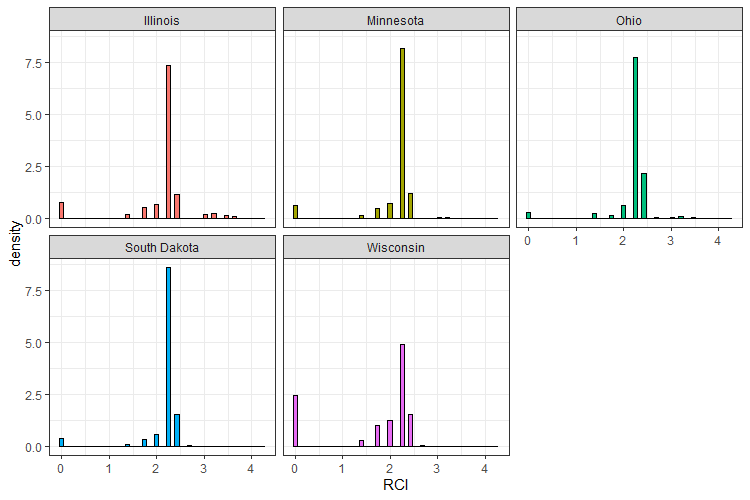
\includegraphics[scale = 0.3]{figures/rci_histograms_corn.png}
        \caption{RCI histograms per state (2010-2020)}
        \label{fig:rci_hist} 
        \end{figure}
        \end{column}%
        \hfill%
        \begin{column}{.5\textwidth}
        \begin{figure}[H]
        \centering
        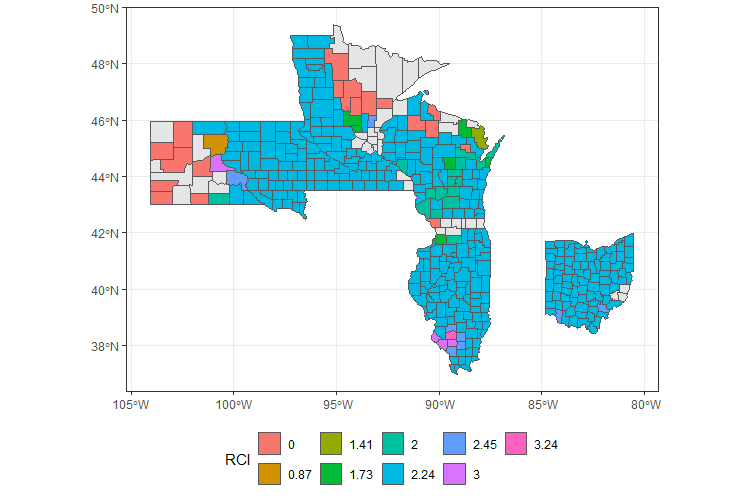
\includegraphics[scale = 0.35]{figures/rci_map_corn.png}
        \caption{Median RCI map}
        \label{fig:rci_map} 
        \end{figure}
        \end{column}%
    \end{columns}
\end{frame}

\begin{frame}{Model 1: RCI as a continuous variable}
    
\begin{table}[H]
   \caption{\label{tab:corn_rci} Rotation Complexity and corn yields}
   \bigskip
   \centering
   \begin{tabular}{lcc}
      \toprule
       & \multicolumn{2}{c}{corn\_yield}\\
                                      & No controls             & Weather and soil controls \\   
                                      & (1)                     & (2)\\  
      \midrule 
      RCI = 1.41                      & 0.4057 (0.8041)         & 0.6237 (0.7213)\\   
      RCI = 1.73                      & -2.035$^{***}$ (0.6712) & -2.037$^{***}$ (0.6014)\\   
      RCI = 2                         & 0.0377 (0.5986)         & -0.5767 (0.5867)\\   
      RCI = 2.24                      & 0.5905 (0.6741)         & -0.5664 (0.6785)\\   
      RCI = 2.45                      & 0.6316 (0.7670)         & -0.1331 (0.7103)\\   
      RCI = 2.65                      & 1.751$^{**}$ (0.7580)   & 0.6746 (0.7601)\\   
      RCI = 2.74                      & -1.520 (1.273)          & 2.421$^{**}$ (1.215)\\   
      RCI = 3                         & 1.204 (1.348)           & -0.1339 (1.126)\\   
      RCI = 3.24                      & 5.085$^{***}$ (1.126)   & 1.733$^{*}$ (0.9865)\\   
      RCI = 3.46                      & 11.91$^{***}$ (1.481)   & 3.963$^{***}$ (1.509)\\   
      RCI = 3.74                      & 10.60$^{***}$ (1.775)   & 3.860$^{**}$ (1.581)\\   
      RCI = 4                         & 15.65$^{***}$ (1.926)   & 7.844$^{***}$ (1.931)\\   
       \\
      Observations                    & 1,581,271               & 1,581,271\\  
      R$^2$                           & 0.81129                 & 0.83643\\  
      Within R$^2$                    & 0.00408                 & 0.13675\\  
       \\
      tile\_field\_ID fixed effects   & $\checkmark$            & $\checkmark$\\   
      year fixed effects              & $\checkmark$            & $\checkmark$\\   
      \bottomrule
   \end{tabular}
\end{table}



\end{frame}

\begin{frame}{Model 1: RCI as a continuous variable}
    \begin{wideitemize}
        \item All coefficients have the expected sign, except for the third moment.
        \item A negative value on $u^{3}$ implies that an increase in rotation diversity decreases the skewness of the distribution, making it more left-skewed and increasing the risk of losses, but the effect is not significant.
        \item The effect on the coefficient of variation is positive but nonsignificant as well.
        \item An increase in rotational complexity leads to higher yields and decreased variance, but the magnitudes of both changes are small.
    \end{wideitemize}
\end{frame}

\begin{frame}{Model 2: Binned RCI}
    \begin{figure}[H]
    \centering
    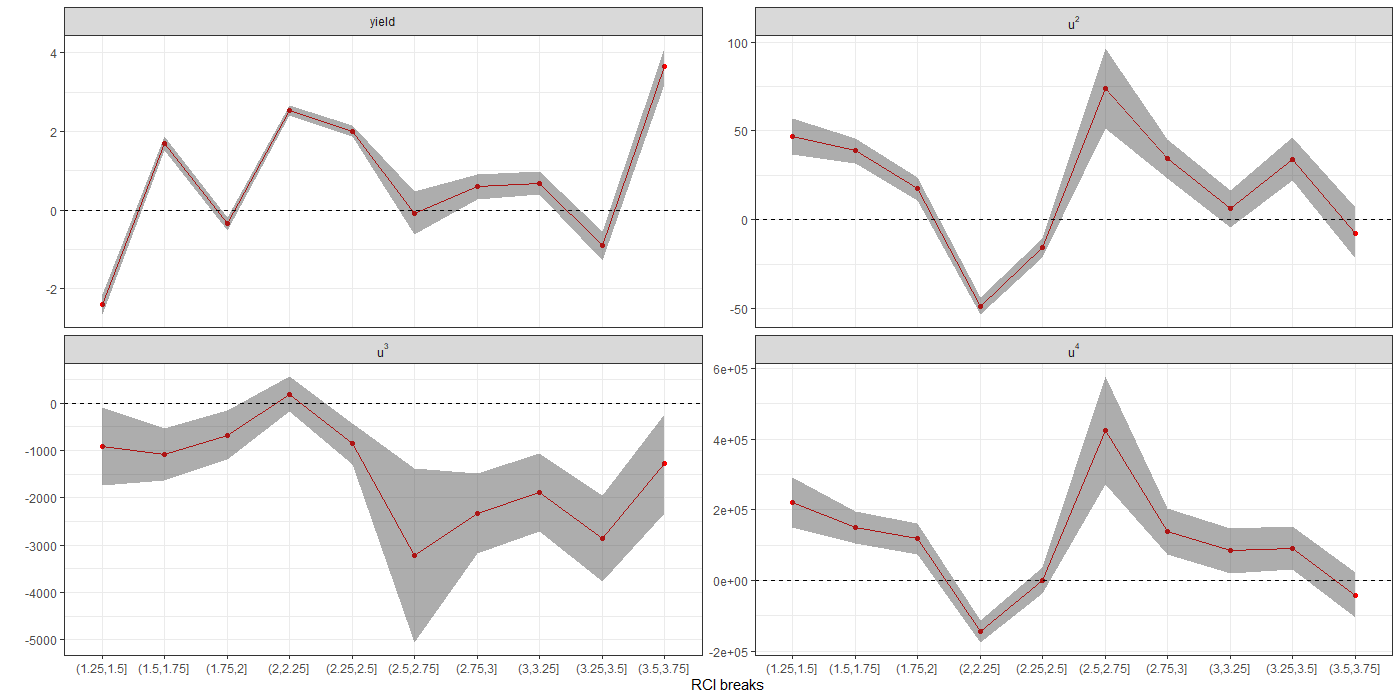
\includegraphics[scale = 0.3]{figures/rci_breaks.png}
    \caption{Effect of RCI on the first four moments of $f(y|X,Z)$}
    \label{fig:rci_breaks} 
    \end{figure}
\end{frame}

\begin{frame}{Model 2: Binned RCI}
   \begin{wideitemize}
       \item We split the RCI into equally spaced bins of width 0.25, keeping zero (corn monoculture) as the base category.
       \item We removed the top two highest categories due to a lack of observations.
       \item Higher RCI increases yields and decreases yields variance only for a number of bins, then the effect reverses.
       \item Notice the singularity of bin $[2,2.5)$, this is where the perfect corn/soy rotations are located.
   \end{wideitemize}
\end{frame}

\begin{frame}{Model 3: individual rotation patterns}
    \begin{wideitemize}
        \item We include rotation patterns as a list of crops detected in the last 6 years (1: corn, 2: soybeans). 
        \item The terminal crop is always corn
        \item Example: "1-2-1-2-1-2" means corn (last year) preceded by soy (previous year), then by corn, and so on.
        \item The base category is again corn monoculture ("1-1-1-1-1-1").
        \item Few rotation patterns "beat" monoculture, all of them include a recent rotation of soy, and no repeated soy harvests.
    \end{wideitemize}
\end{frame}

\begin{frame}{Model 3: individual rotation patterns}
    \begin{figure}[H]
    \centering
    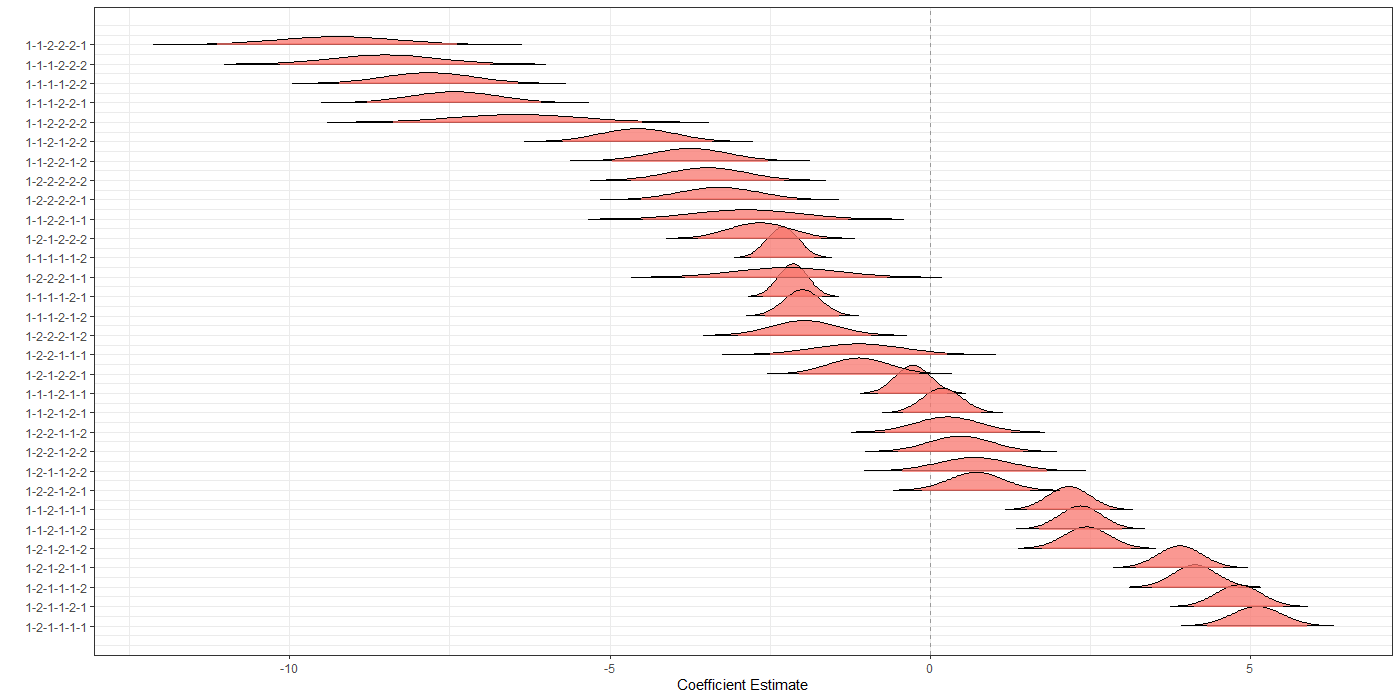
\includegraphics[scale = 0.35]{figures/crop_rotation_arranged.png}
    \caption{Response of yields to rotation sequences}
    \label{fig:crop_rotation_yields} 
    \end{figure}
\end{frame}

\begin{frame}{Model 4: individual rotation patterns (split by categories)}
    \begin{figure}[H]
    \centering
    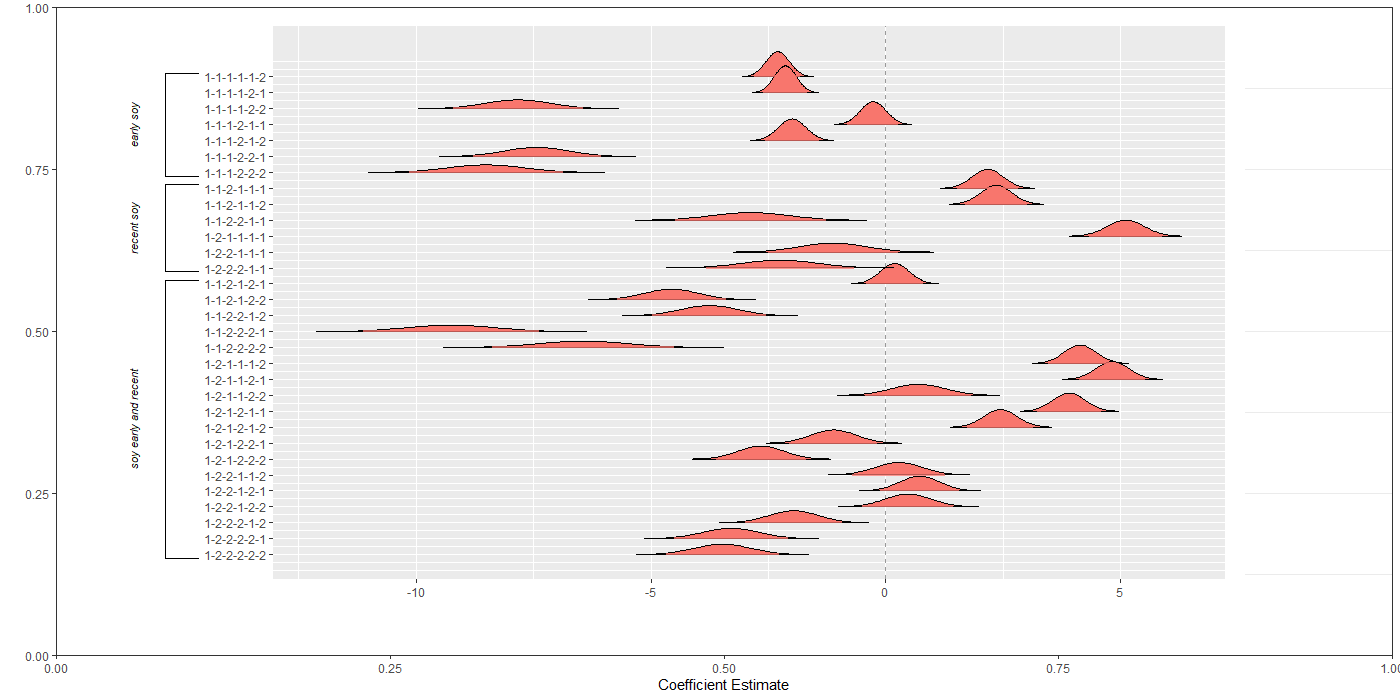
\includegraphics[scale = 0.35]{figures/crop_rotation_types.png}
    \caption{Response of yields to rotation sequences}
    \label{fig:crop_rotation_types} 
    \end{figure}
\end{frame}

\begin{frame}{Model 4: individual rotation patterns (ordered by RCI values)}
    \begin{figure}[H]
    \centering
    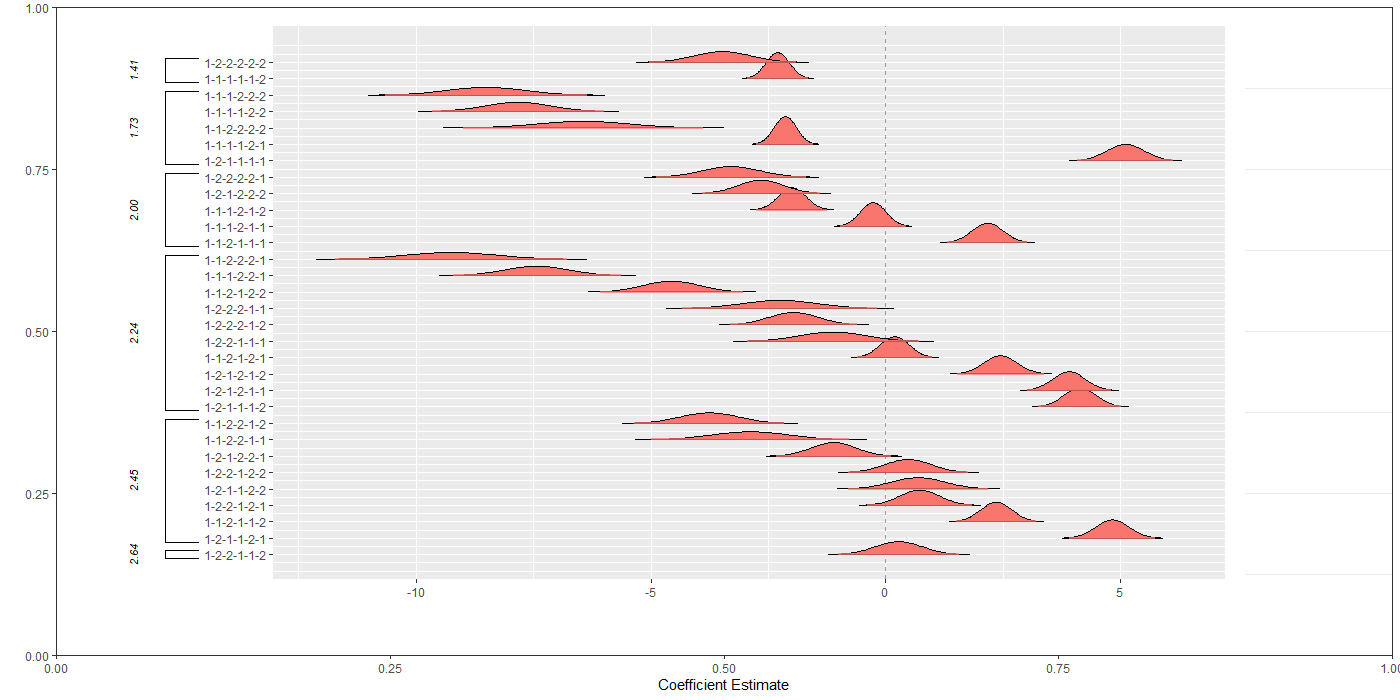
\includegraphics[scale = 0.35]{figures/rci_coeff.png}
    \caption{Response of yields to rotation sequences}
    \label{fig:crop_rotation_yields} 
    \end{figure}
\end{frame}

\begin{frame}{A few takeaways}
    \begin{wideitemize}
        \item Several rotation patterns have the same RCI value, but vastly different impacts on yields.
        \item RCI is defined in terms of turnover frequencies, and it is "designed" to penalize lower rotation frequencies with fewer crops, with just two of them, it leads to strange results.
        \item We find that rotating with soy in the last three years leads to higher corn yields.
        \item Similarly, two (or more) consecutive soy years lead to lower corn yields in the present.
        \item Alternatives?
    \end{wideitemize}
\end{frame}

\begin{frame}{Additional variables}
    
\begingroup
\centering
\scalebox{0.65}{
\begin{tabular}{lcccccc}
\footnotesize
   \tabularnewline \midrule \midrule
   Dependent Variables: & yield          & $u^{2}$       & yield          & $u^{2}$        & yield         & $u^{2}$\\   
   \midrule
   \emph{Variables}\\
   cons\_soy            & -3.386$^{***}$ & 59.61$^{***}$ &                &                &               &   \\   
                        & (0.0514)       & (2.020)       &                &                &               &   \\   
   timing $=$ earlysoy  &                &               & -1.869$^{***}$ & 30.37$^{***}$  &               &   \\   
                        &                &               & (0.0821)       & (3.210)        &               &   \\   
   timing $=$ recentsoy &                &               & 3.127$^{***}$  & 5.930$^{*}$    &               &   \\   
                        &                &               & (0.0815)       & (3.210)        &               &   \\   
   timing $=$ soyboth   &                &               & 2.420$^{***}$  & -47.04$^{***}$ &               &   \\   
                        &                &               & (0.0622)       & (2.405)        &               &   \\   
   cs                   &                &               &                &                & 3.053$^{***}$ & -74.02$^{***}$\\   
                        &                &               &                &                & (0.0390)      & (1.524)\\   
   Controls             & Yes            & Yes           & Yes            & Yes            & Yes           & Yes\\  
   \midrule
   \emph{Fixed-effects}\\
   year                 & Yes            & Yes           & Yes            & Yes            & Yes           & Yes\\  
   fips                 & Yes            & Yes           & Yes            & Yes            & Yes           & Yes\\  
   \midrule
   \emph{Fit statistics}\\
   R$^2$                & 0.66641        & 0.06080       & 0.66662        & 0.06102        & 0.66661       & 0.06164\\  
   Observations         & 2,691,945      & 2,691,945     & 2,691,945      & 2,691,945      & 2,691,945     & 2,691,945\\  
   \midrule \midrule
   \multicolumn{7}{l}{\emph{Heteroskedasticity-robust standard-errors in parentheses}}\\
   \multicolumn{7}{l}{\emph{Signif. Codes: ***: 0.01, **: 0.05, *: 0.1}}\\
\end{tabular}}
\par\endgroup



\end{frame}

\begin{frame}{Additional variables}
    \begin{wideitemize}
        \item We can include different dummies to account for the impact of "early" vs "late" soy harvests, two or more consecutive soy years, and soy followed by corn in year "-1".
        \item "Early soy": if there was one or more soy harvests in years -5 to -3, "Later soy" if there was one or more soy harvests in years -1 to -3, "both" if no clear pattern emerges.
        \item Having an early soy rotation has a positive impact on yields (relative to monoculture).
        \item "cons\_soy": two or more consecutive soy harvests, it is correlated with lower corn yields, regardless of its timing.
    \end{wideitemize}
\end{frame}

\begin{frame}{Next steps}
    \begin{wideitemize}
        \item Bootstraped standard errors (high memory requirement).
        \item Additional rotation patterns (wheat as a third crop, other functional groups)
        \item Include Soy data.
        \item Use full data set (5X larger).
        \item Address endogeneity issues (unobserved?)
        \item What are the crop insurance implications of our results?
    \end{wideitemize}
\end{frame}

\begin{frame}{}
	\centering \Huge
	\emph{Thank You!}
\end{frame}
	
\begin{frame}[allowframebreaks]{References}
	\bibliography{bibliography.bib}	
\end{frame}	
\end{document}
